\begin{pastexam}[label={px:ncku-109-comm-ds-02}]{成大電通所 109 學年度 第 2 題}
（手算追蹤）

The following array represents a complete binary tree. Adjust it to be a min heap by
\textbf{showing each step.} (15 points)

\begin{center}
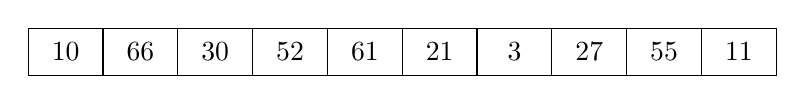
\begin{tikzpicture}[x=9.5mm,y=6mm]
\foreach \v [count=\i from 0] in {10,66,30,52,61,21,3,27,55,11}{
  \draw (\i,0) rectangle ++(1,1);
  \node at (\i+0.5,0.5) {\v};
}
\end{tikzpicture}
\end{center}
\end{pastexam}

\begin{pastsoln}
用由下而上建堆積（資結書第~8.2~節）：陣列從 $1$ 編號，$n = 10$，從最後一個有子節點的位置
$\lfloor n/2 \rfloor = 5$ 往回到 $1$，每個位置做一次下沉（和較小的子節點比，比它大就交換，繼續往下）。

原來的樹：
\begin{center}
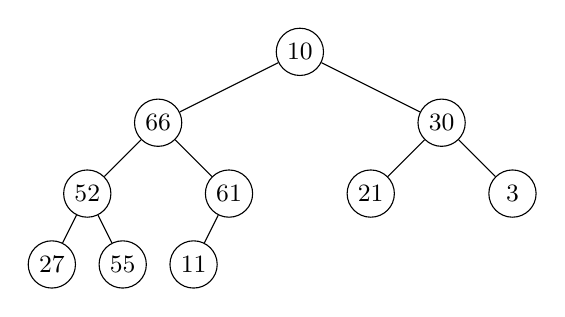
\begin{tikzpicture}[level distance=9mm,
  level 1/.style={sibling distance=36mm},level 2/.style={sibling distance=18mm},
  level 3/.style={sibling distance=9mm},
  every node/.style={circle,draw,inner sep=0pt,minimum size=6mm,font=\small}]
\node {10}
  child {node {66} child {node {52} child {node {27}} child {node {55}}}
                   child {node {61} child {node {11}} child[missing]}}
  child {node {30} child {node {21}} child {node {3}}};
\end{tikzpicture}
\end{center}

\begin{center}
\small
\begin{tabular}{clc}
\toprule
步驟 & 動作 & 之後的陣列 $A[1..10]$ \\
\midrule
開始 & & 10, 66, 30, 52, 61, 21, 3, 27, 55, 11 \\
$i = 5$ & $61$ 的子節點 $11$；$61 > 11$，交換 & 10, 66, 30, 52, \textbf{11}, 21, 3, 27, 55, \textbf{61} \\
$i = 4$ & $52$ 的子節點 $27, 55$，較小 $27$；交換 & 10, 66, 30, \textbf{27}, 11, 21, 3, \textbf{52}, 55, 61 \\
$i = 3$ & $30$ 的子節點 $21, 3$，較小 $3$；交換 & 10, 66, \textbf{3}, 27, 11, 21, \textbf{30}, 52, 55, 61 \\
$i = 2$ & $66$ 和子節點 $27, 11$ 的較小者 $11$ 交換（到位置 $5$）； & \\
 & \quad 再和子節點 $61$ 交換（到位置 $10$） & 10, \textbf{11}, 3, 27, \textbf{61}, 21, 30, 52, 55, \textbf{66} \\
$i = 1$ & $10$ 和子節點 $11, 3$ 的較小者 $3$ 交換（到位置 $3$）； & \\
 & \quad 子節點 $21, 30$ 都比 $10$ 大，停 & \textbf{3}, 11, \textbf{10}, 27, 61, 21, 30, 52, 55, 66 \\
\bottomrule
\end{tabular}
\end{center}

結果是 $3, 11, 10, 27, 61, 21, 30, 52, 55, 66$：
\begin{center}
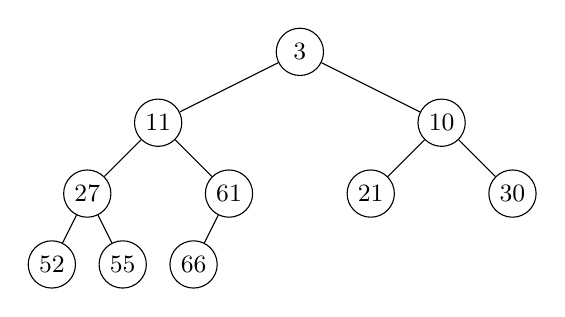
\begin{tikzpicture}[level distance=9mm,
  level 1/.style={sibling distance=36mm},level 2/.style={sibling distance=18mm},
  level 3/.style={sibling distance=9mm},
  every node/.style={circle,draw,inner sep=0pt,minimum size=6mm,font=\small}]
\node {3}
  child {node {11} child {node {27} child {node {52}} child {node {55}}}
                   child {node {61} child {node {66}} child[missing]}}
  child {node {10} child {node {21}} child {node {30}}};
\end{tikzpicture}
\end{center}
檢查：每個父節點都不大於子節點（$3 \le 11, 10$；$11 \le 27, 61$；$10 \le 21, 30$；$27 \le 52, 55$；
$61 \le 66$），是最小堆積。

如果改成「從空堆積開始依序插入這 $10$ 個數」，每次插入後往上調整，最後的陣列會不一樣（是
$3, 11, 10, 52, 27, 30, 21, 66, 55, 61$）。 題目是把現成的陣列調整成堆積，用由下而上的做法，時間
$O(n)$。
\end{pastsoln}
